
\begin{figure}
\centering
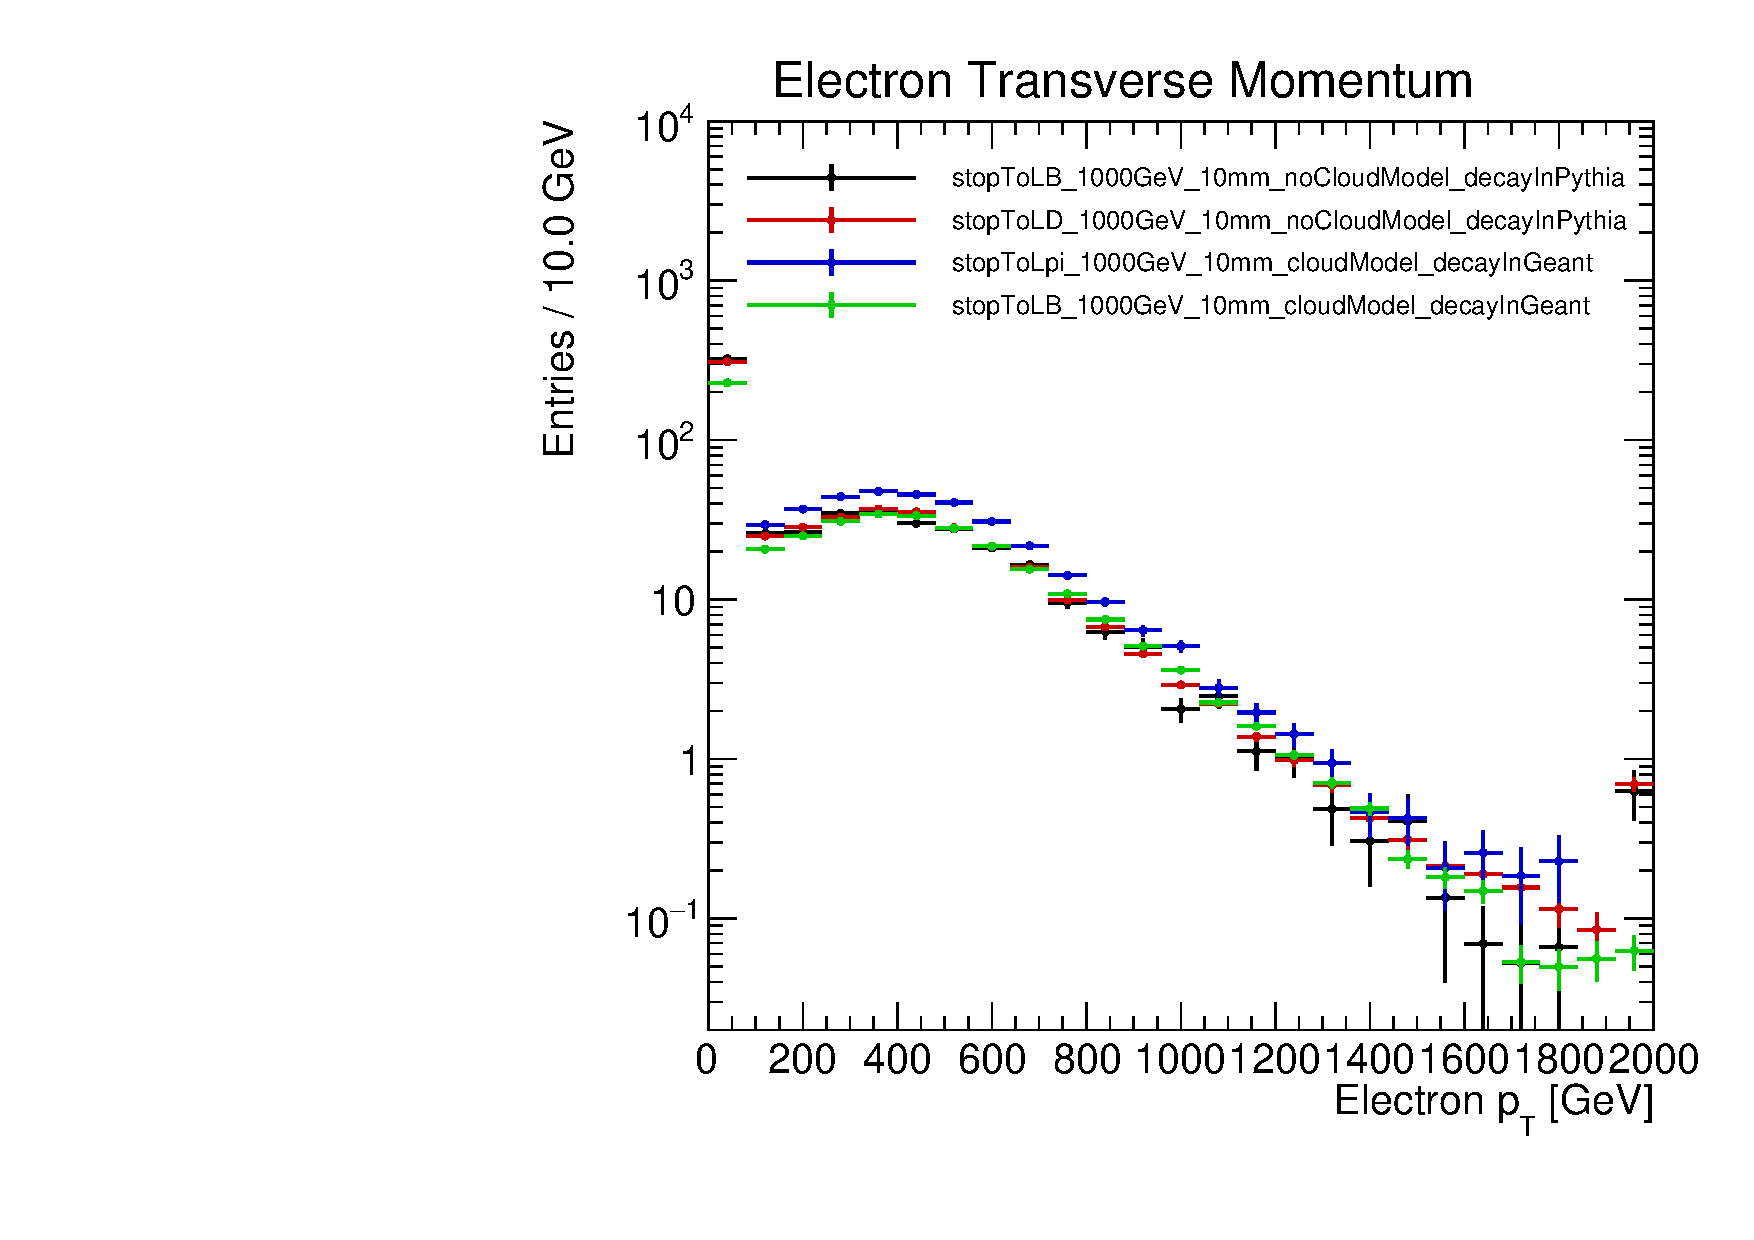
\includegraphics[width=0.35\textwidth]{figures/r_hadrons/e_pt_1000GeV_10mm.pdf}
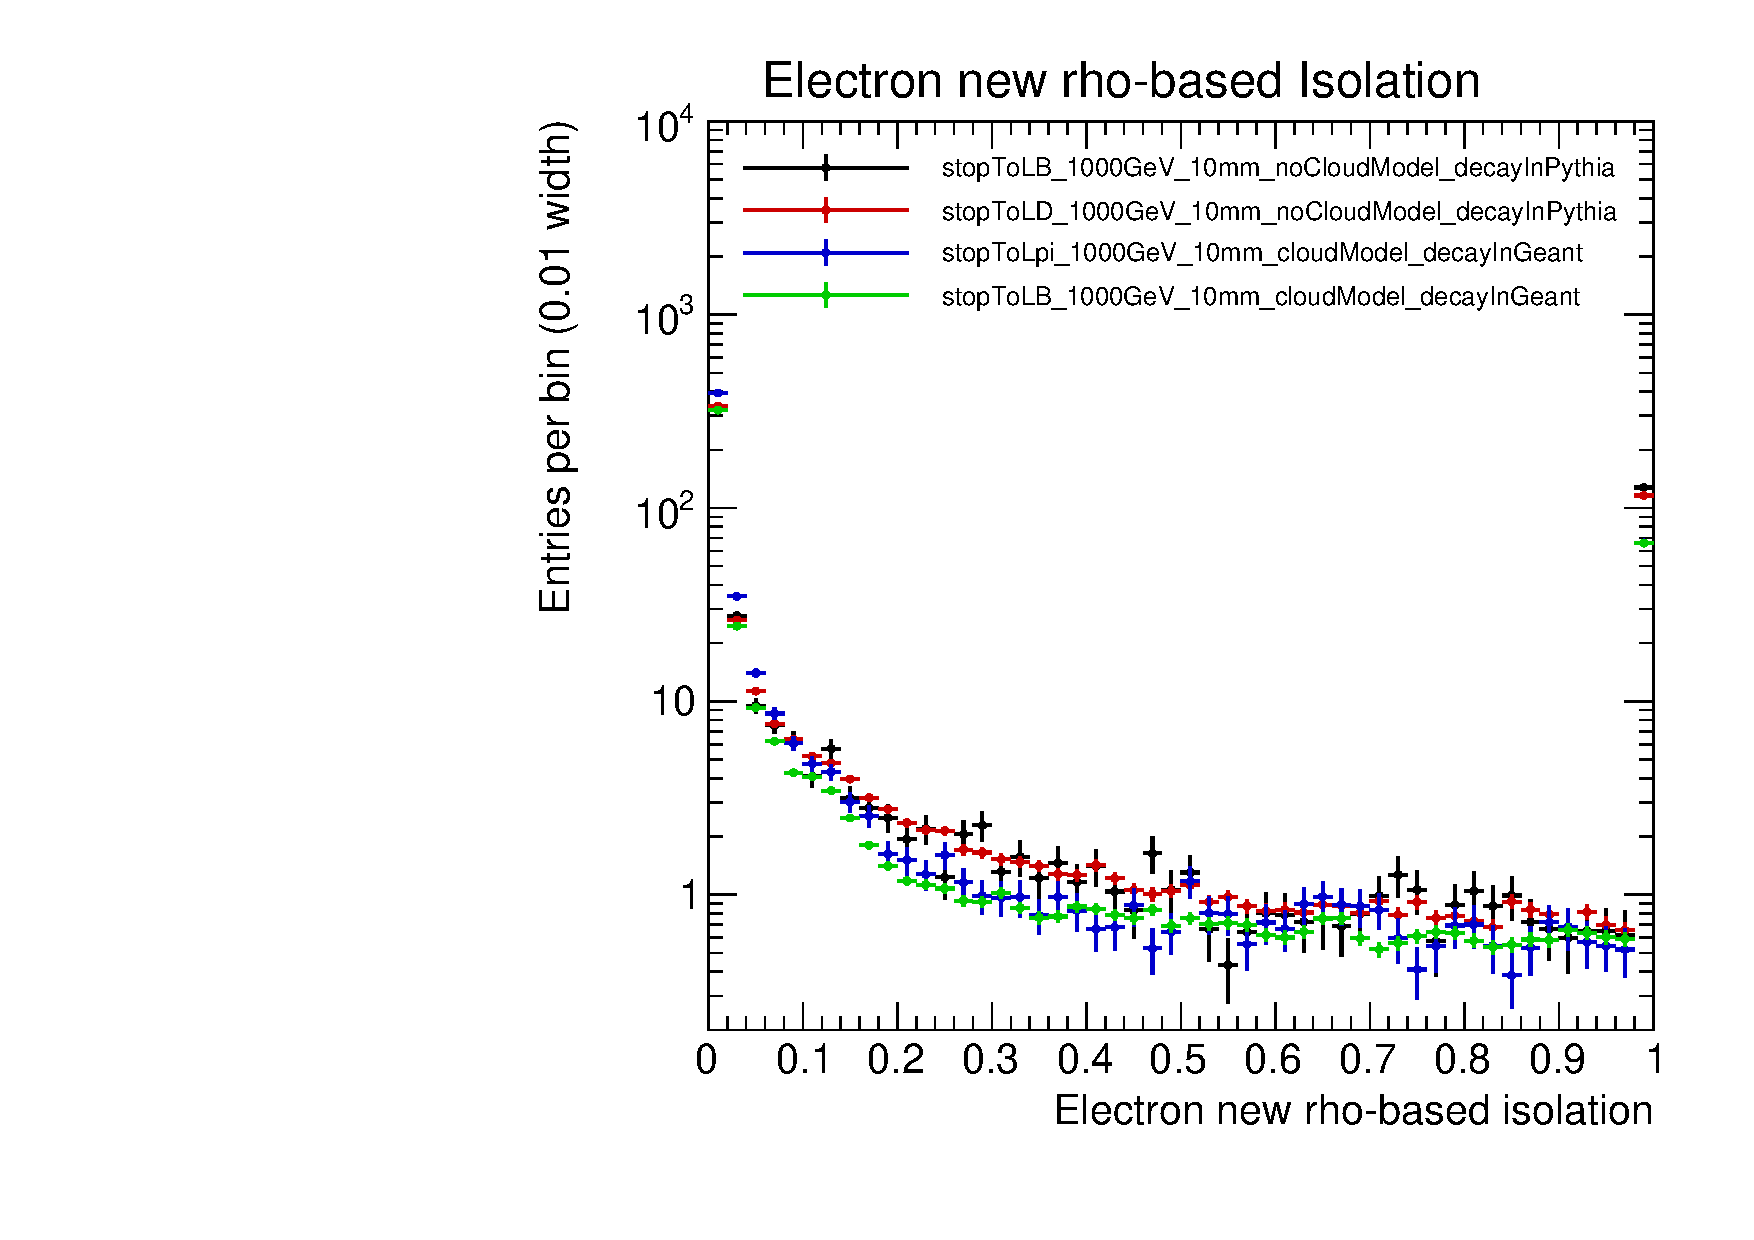
\includegraphics[width=0.35\textwidth]{figures/r_hadrons/e_iso_1000GeV_10mm.pdf}
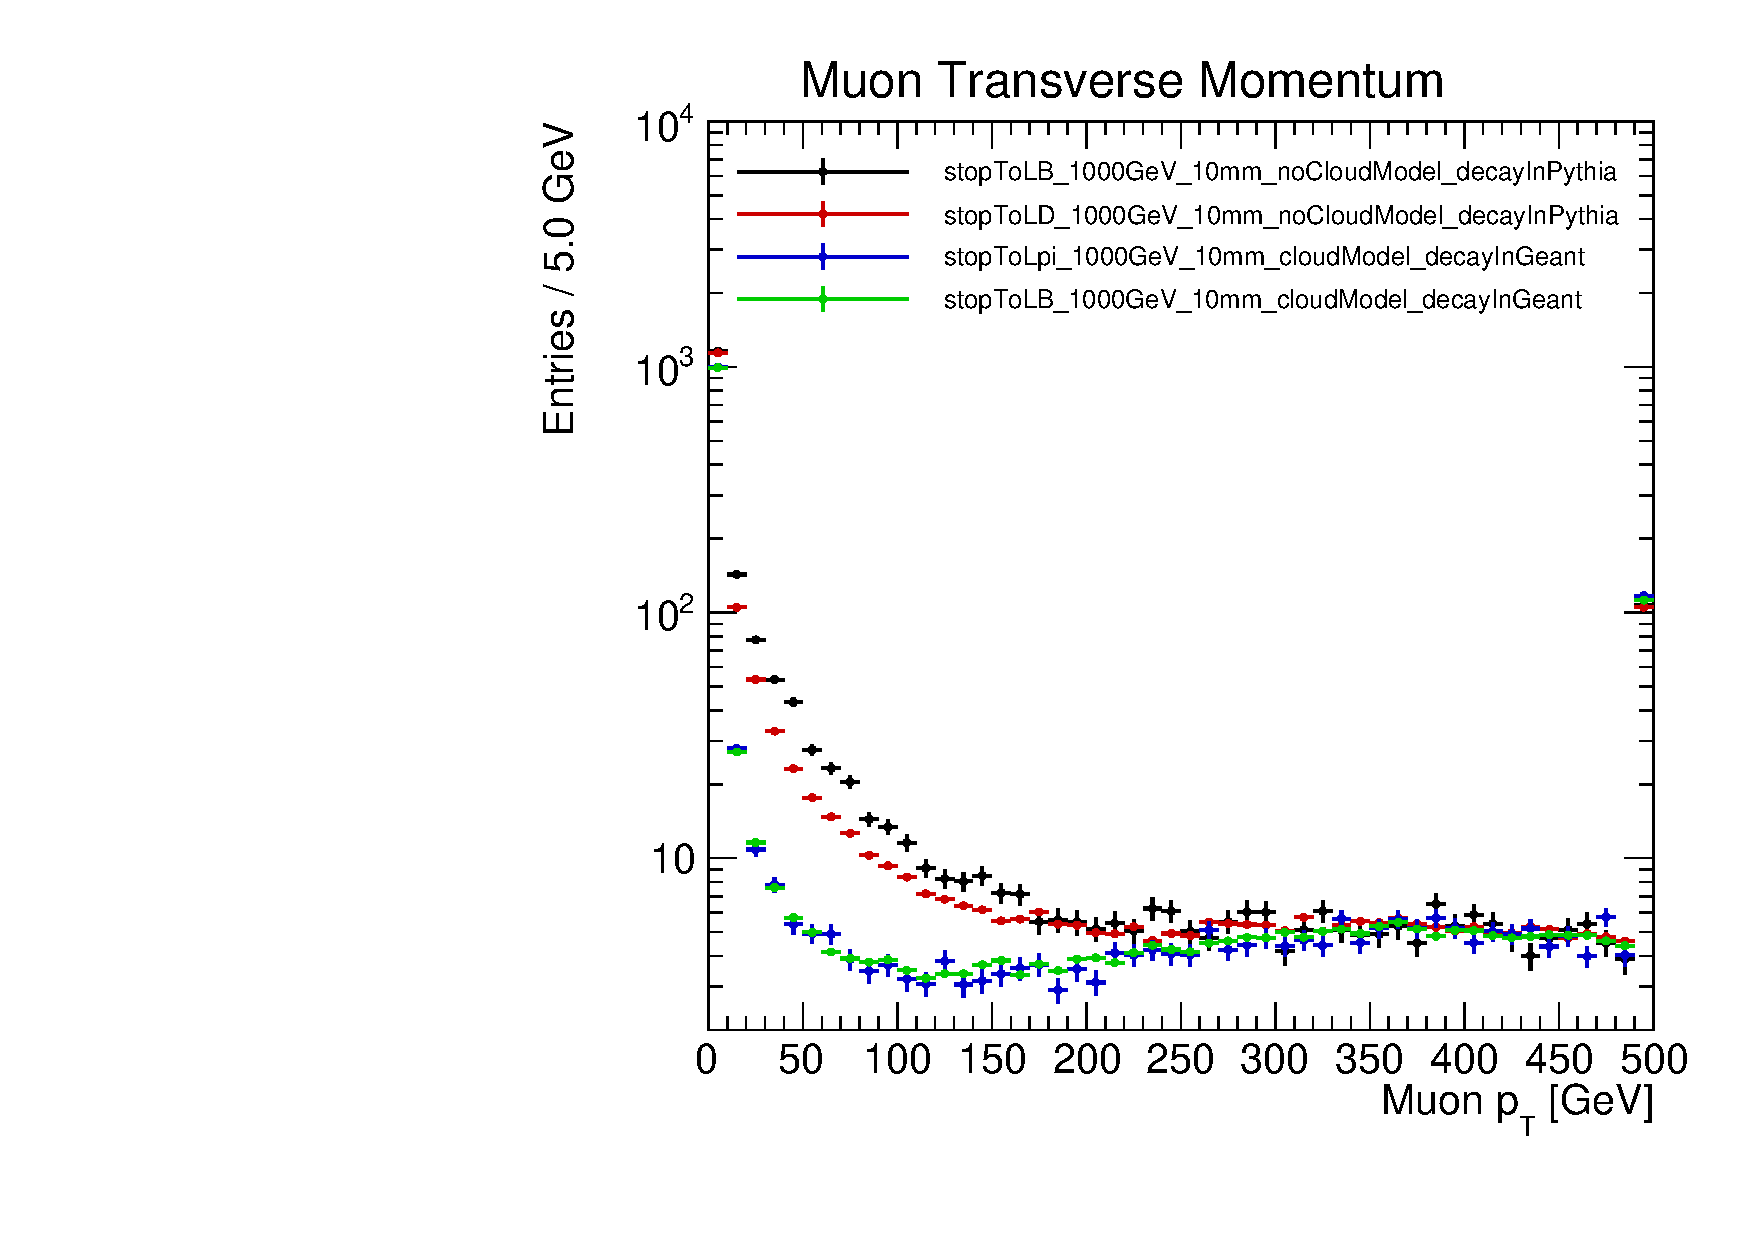
\includegraphics[width=0.35\textwidth]{figures/r_hadrons/mu_pt500_1000GeV_10mm.pdf}
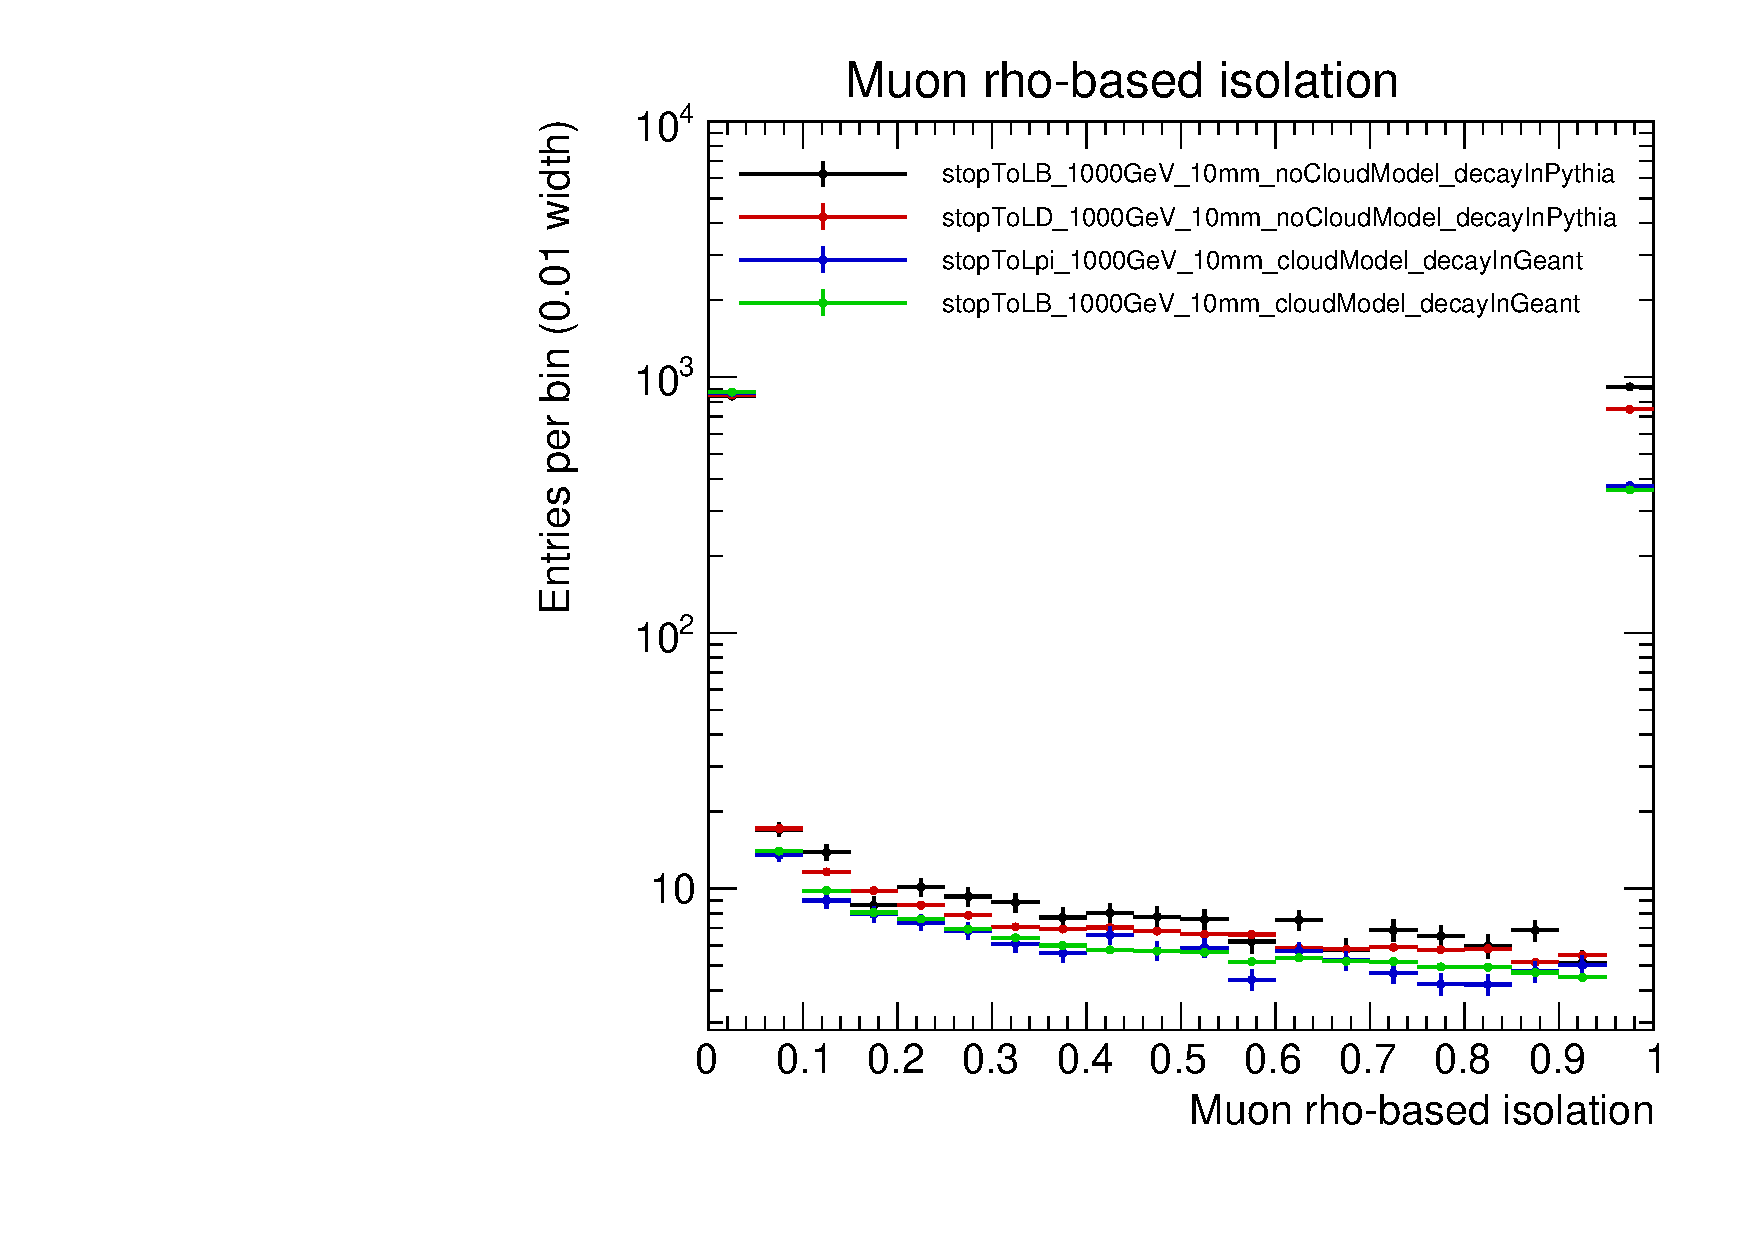
\includegraphics[width=0.35\textwidth]{figures/r_hadrons/mu_iso_1000GeV_10mm.pdf}
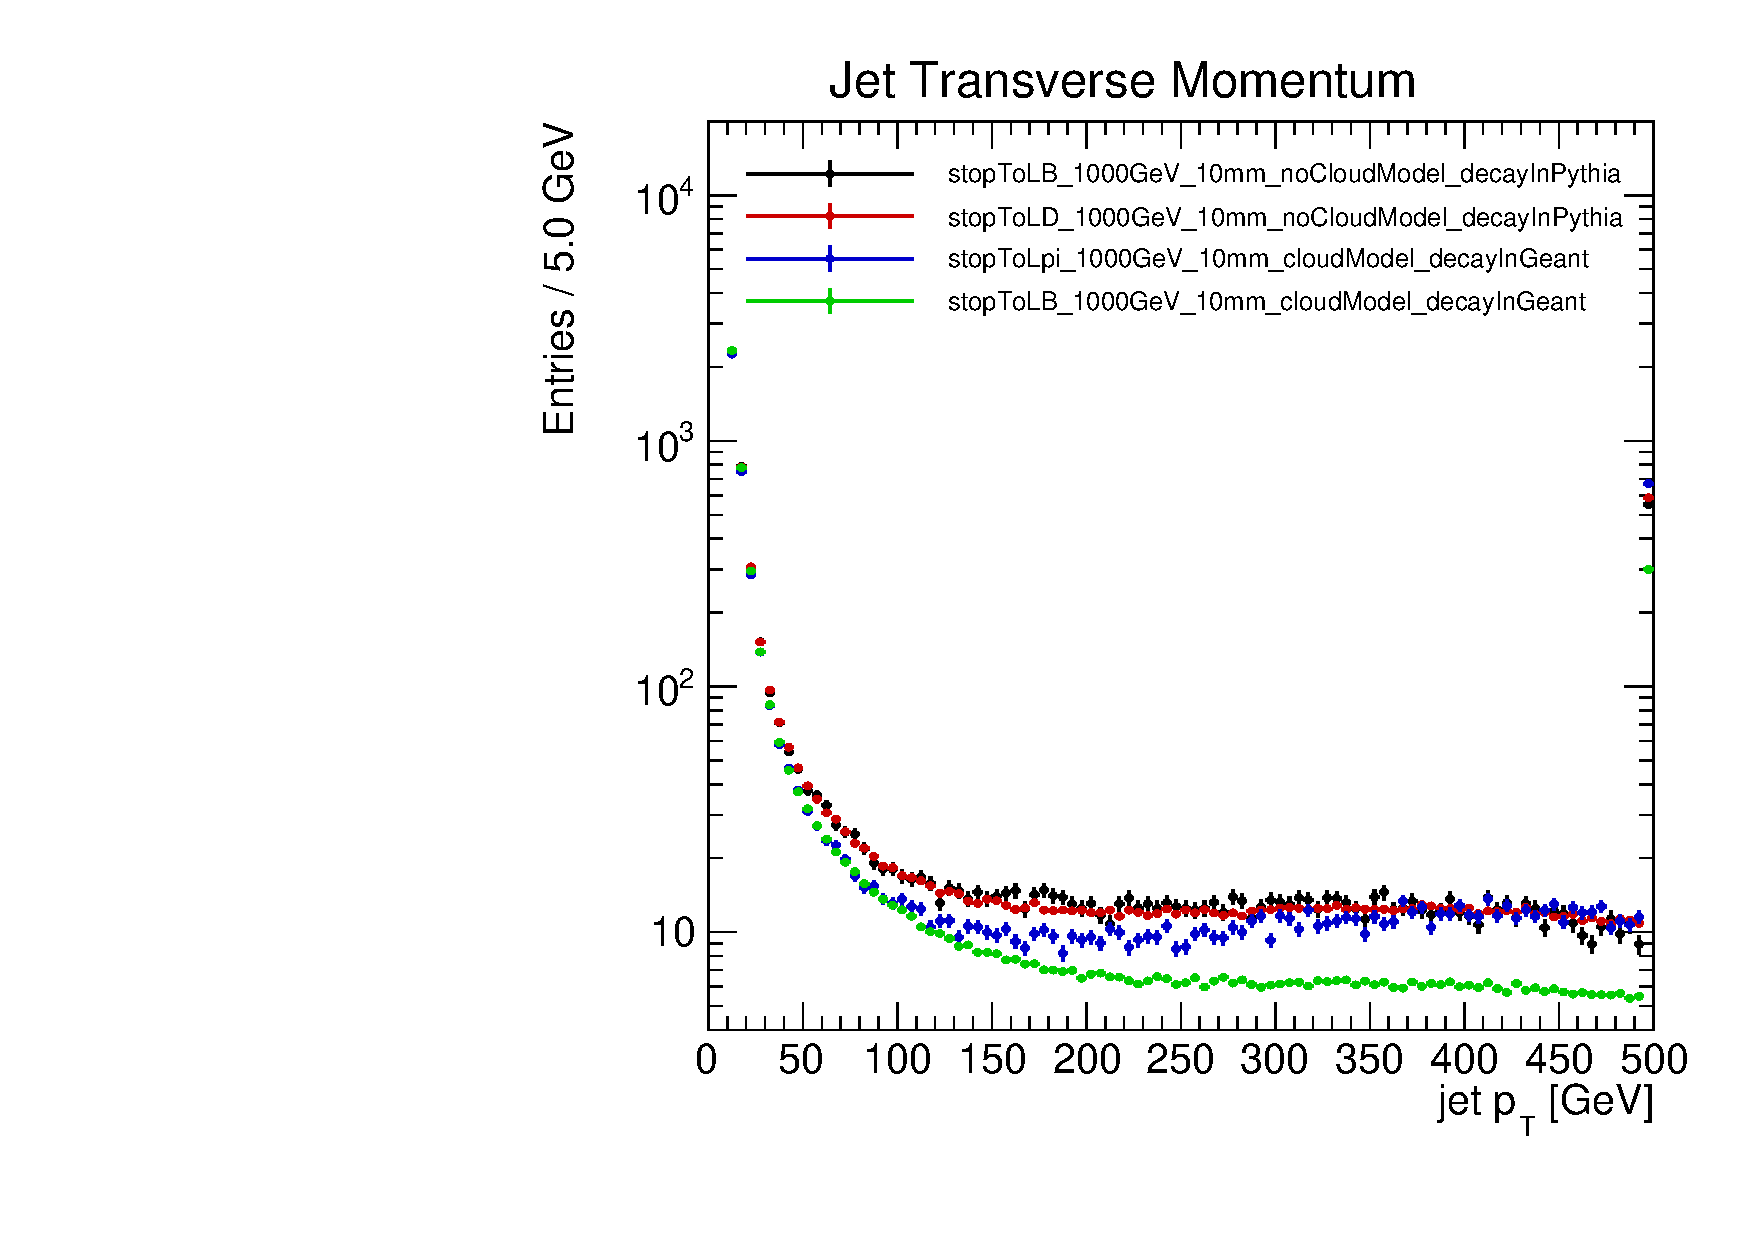
\includegraphics[width=0.35\textwidth]{figures/r_hadrons/jet_pt_1000GeV_10mm.pdf}
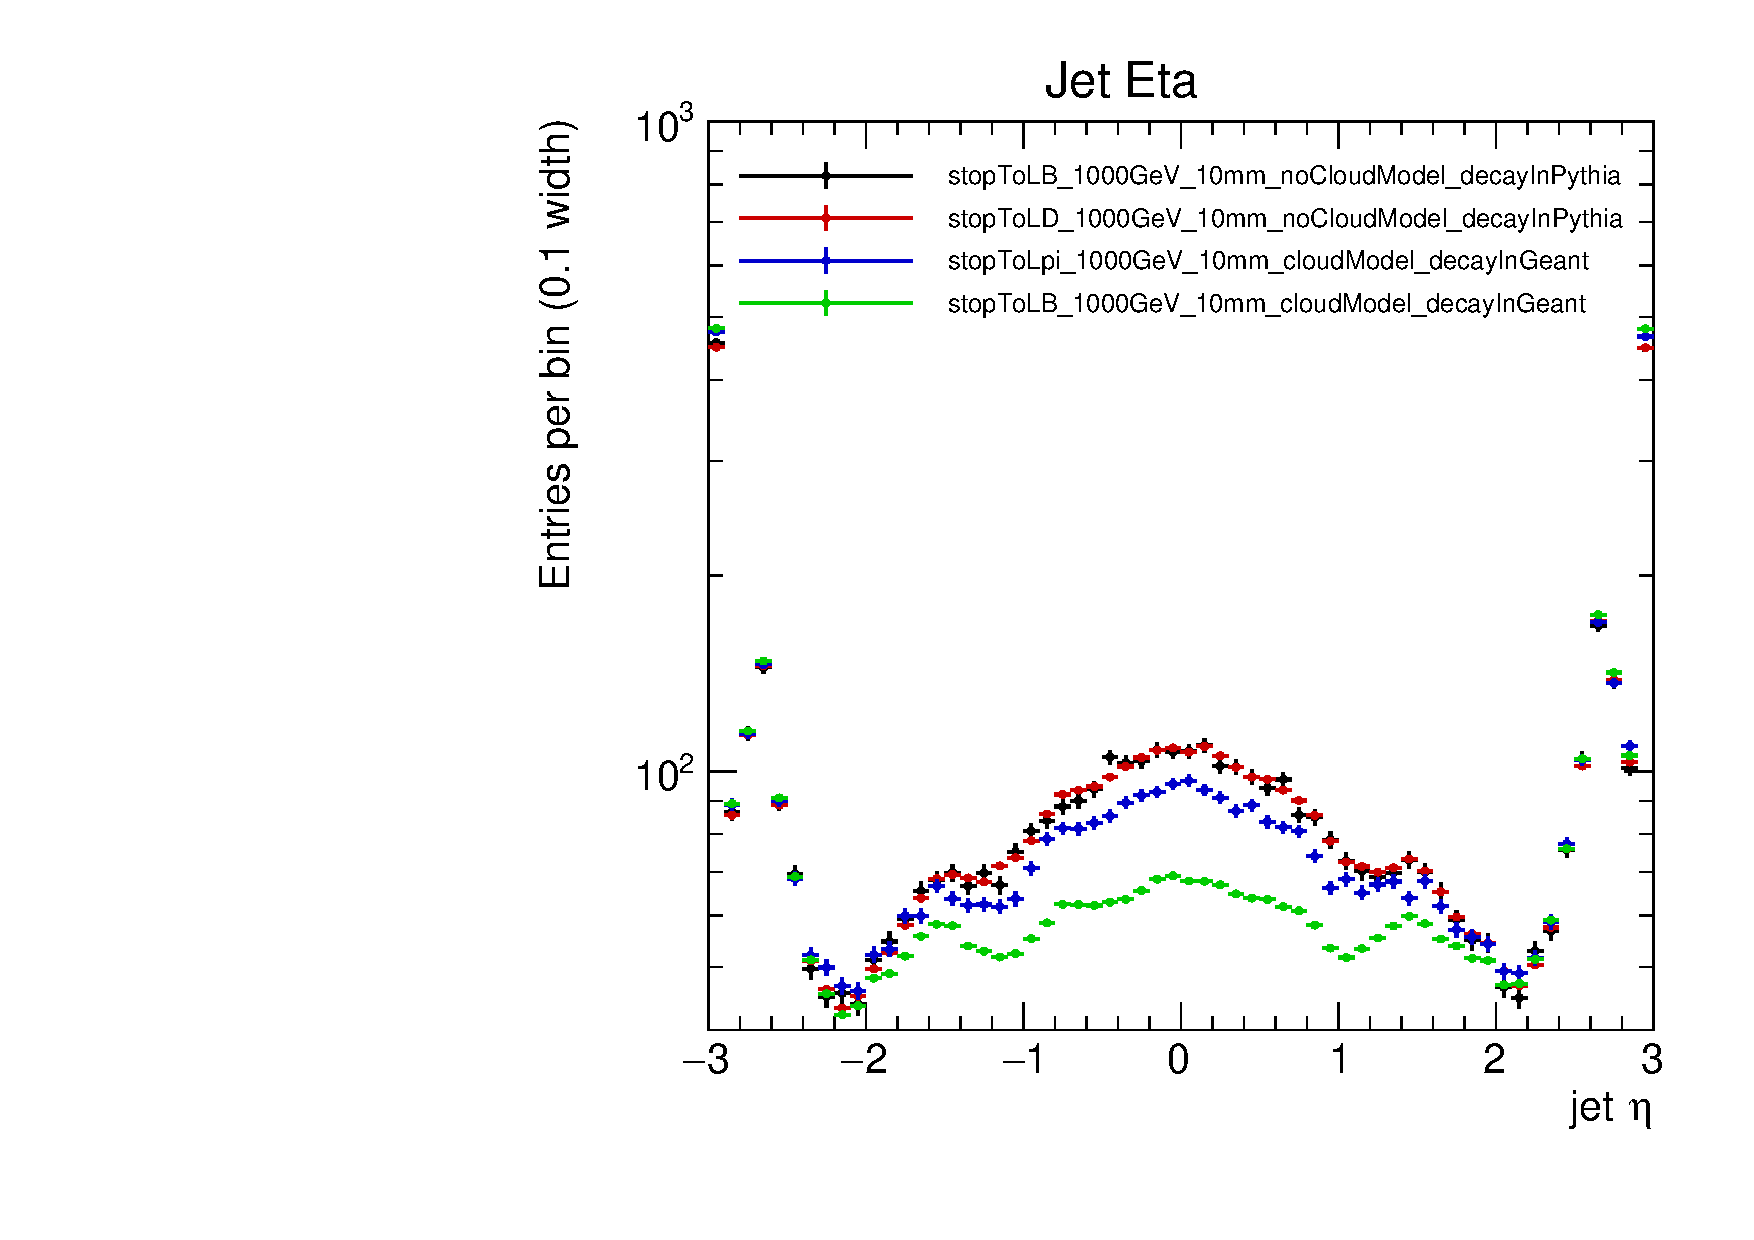
\includegraphics[width=0.35\textwidth]{figures/r_hadrons/jet_eta_1000GeV_10mm.pdf}
\caption{
Kinematic distributions of electrons (top), muons (middle), and jets (bottom) before any selection is applied for four signal samples in which the top squark mass and proper decay length are 1000\GeV and 1\cm. In the sample corresponding to the black (red) curves, R-hadron material interactions are not modeled, but the top squark decay is performed in \PYTHIA and the resulting b (d) quark produces a jet. In the samples corresponding to the blue and green curves, the R-hadron material interactions and decay are modeled with \GEANTfour. In the sample corresponding to the blue curves, the R-hadron decays to a lepton and a neutral pion, and in the sample corresponding to the green curves, the R-hadron decays to a lepton and a non-physical final-state quark. In each plot, the rightmost bin contains overflow entries.
}
\label{r_hadrons_no_selection}
\end{figure}